\documentclass[11pt,a4paper]{article}
\usepackage[utf8]{inputenc}
\usepackage[spanish,es-tabla]{babel}
\usepackage{amsmath}
\usepackage{amsfonts}
\usepackage{amssymb}
\usepackage{graphicx}
\usepackage{natbib}
\usepackage{lineno}
\usepackage{ragged2e}
\usepackage{multicol}
\setlength\columnsep{38pt}
\usepackage{enumerate} 
\usepackage[left=2.8cm,top=2.3cm,right=2.8cm,bottom=2.3cm]{geometry} 
\usepackage{fancyhdr}
\usepackage{url}
\usepackage{float}


\begin{document}
		
		\begin{center}
			\huge \textbf{Sistema de Recomendacion: Airbnb} 
		\end{center}
		\vspace{\baselineskip}
		\begin{center}
			
\includegraphics[scale=0.37]{./Imagenes/logo}
		\end{center}
		\vspace{\baselineskip}
		\begin{multicols}{2}
			\small
			\begin{center}
				Nelia Escalante Marón\\
				2014049551\\
				UPT Ingeniería de Sistemas\\
				Tacna, Perú\\
				
				\vspace{\baselineskip}
				
				Yerson Coaquira Calizaya\\
				2015053225\\
				UPT Ingeniería de Sistemas\\  
				Tacna, Perú\\   
				\columnbreak              
				
				Flor Condori Gutierrez\\
				2015053227\\
				UPT Ingeniería de Sistemas\\  
				Tacna, Perú\\                 
				
				           
			\end{center}
			\normalsize			
		\end{multicols}
		\vspace{\baselineskip}
		\vspace{\baselineskip}
		\vspace{\baselineskip}

		\textbf{\textit{\large Resumen}}\rule[1.5mm]{5mm}{0.1mm}		
		Un sistema de recomendación es un sistema inteligente que proporciona a los usuarios una serie de sugerencias personalizadas (recomendaciones) sobre un determinado tipo de elementos (ítems). Los sistemas de recomendación estudian las características de cada usuario y mediante un procesamiento de los datos, encuentra un subconjunto de ítems que pueden resultar de interés para el usuario.\\
		\\
		En los últimos años y debido principalmente a la sobre carga de información que tenemos en internet, han proliferado los sistemas de recomendación, los cuales proporcionan a los usuarios, información, productos, etc. que puedan ser del interés del usuario, tras realizar un "estudio" de su perfil, su gusto e incluso de la forma en la que el usuario navega por internet.
				
		\vspace{\baselineskip}
		
		\textbf{\textit{\large Abstract}}\rule[1.5mm]{5mm}{0.1mm} 		
		\textit{
			A recommendation system is an intelligent system that provides users with a series of personalized suggestions (recommendations) about a certain type of elements (items). The recommendation systems study the characteristics of each user and through a processing of the data, find a subset of items that may be of interest to the user.
			In recent years and mainly due to the overload of information that we have on the Internet, recommendation systems have proliferated, which provide users, information, products, etc. that may be of interest to the user, after conducting a "study "of your profile, your taste and even the way in which the user browses the internet.	
			\vspace{\baselineskip}			
		 }				
					
		\rule{150mm}{0.1mm}
		
		\newpage
		
		\section{INTRODUCCION}
		Los sistemas de recomendación pueden definirse como herramientas diseñadas para interactuar con conjuntos de información grandes y complejos con la finalidad de proporcionar al usuario información o ítems que sean de su interés, todo ello de forma automatizada. Su funcionamiento se basa en el empleo de métodos matemáticos y estadísticos capaces de explotar la información previamente almacenada y crear recomendaciones adaptadas a cada usuario. En la actualidad, los sistemas de recomendación son una tecnología implementada en la mayoría de plataformas online como Amazon, Neflix, eBay… ya que han dado muy buenos resultados incrementando las ventas. También están presentes en muchos otros ámbitos, por ejemplo, el de las noticias, mostrando al usuario información que le interesa de forma rápida. La mayoría de sistemas de recomendación se pueden clasificar en tres grupos: basados en contenido, filtrado colaborativos y mixtos (combinación de los dos anteriores).\\
		\\
		El objetivo de los ejemplos mostrados en este documento es facilitar la comprensión de las ideas que hay detrás de algunos de estos sistemas, no persiguen ser una implementación óptima y sofisticada, sino intuitiva. Para sistemas más optimizados pueden emplearse librerías como \textit{recommenderlab}.
		
		\section{MARCO TEORICO}
		
			 \subsection{SISTEMA DE RECOMENDACIÓN}
			 Un sistema de recomendación (SR) muestra resultados de una búsqueda efectiva de información. Encuentra datos precisos que el usuario desea conseguir. Para esto considera datos introducidos o generados a partir del funcionamiento del propio sistema. Un SR sugiere temas o productos fundamentándose en preferencias.\\
			 \\
			 Una de las variables importantes es el volumen de la información, ya que de éste depende el detalle de las recomendaciones. Factores como el tiempo de vida (del elemento a evaluar), el tipo de elemento (películas, gente, artículos, etcétera) y la cantidad generada influyen de manera directa en el momento de la recomendación.\\
			 \\
			 Debido a que mantener un sistema de recomendación es caro, se han considerado diferentes modelos para costear dichos sistemas:
			 	\begin{itemize}
			 		\item El consumidor paga por el servicio.
			 		\item Los anuncios de publicidad mantienen el sistema.
			 		\item El dueño del elemento a evaluar paga por la evaluación de su elemento.
			 	\end{itemize}
		 	
		 		\begin{figure}[H]
		 			\begin{center}
		 				
\includegraphics[scale=0.9]{./Imagenes/img01}		
		 			\end{center}
		 		\end{figure}
	 		
	 		Funciona en dos etapas: La primera es el aprendizaje de lo que me gusta, a través de páginas web, bibliotecas digitales, aplicaciones, o por sistemas de puntuación. Aquí es fundamental la recopilación de información del usuario, para crear un perfil personalizado, pues esto define la calidad de recomendación. La segunda etapa es la recomendación en sí. Envía sugerencias de lo que me puede gustar.
	 		En el aprendizaje la información se obtiene de dos formas:
	 		\begin{enumerate}[i.]
	 			\item Explícita\\
	 			\\
	 			El usuario ingresa sus preferencias directamente. Por ejemplo, al seleccionar un producto de una lista, o llenar un formulario de registro. Si se requiere ser preciso, se presenta la desventaja de realizar demasiadas preguntas. Por lo que surge el riesgo de desinterés o no respuesta
	 			
	 			\item Implícita\\
	 			\\
	 			Se obtiene la información de páginas visitadas, como las redes sociales o tiendas online. Aquí, se registran indirectamente las preferencias. Una forma de hacerlo es analizar la nómina de productos de la tienda, revisar el número de visitas que registra, o mediante el historial de compras. \\
	 			Este método presenta el riesgo de obtener datos erróneos. Por ejemplo, si en una página de comercio electrónico el usuario busca un producto para un tercero, que nada tiene que ver con sus gustos. Se considera que la mejor manera de recopilar información, es de forma combinada, debido a que se reducen los riesgos producidos.\\
	 			\\
	 			Algunos ejemplos de recolección de datos de forma implícitas son:
	 			
	 				\begin{itemize}
	 					\item Guardar un registro de los temas que el usuario ha visto en una tienda en línea.
	 					\item Analizar el número de visitas que recibe un artículo
	 					\item Guardar un registro de los artículos que el usuario ha seleccionado.
	 					\item Obtener un listado de los artículos que el usuario ha seleccionado o visto en su computadora.
	 					\item Analizar las redes sociales de las que el usuario forma parte y de esta manera conocer sus gustos y preferencias.
	 				\end{itemize}
	 		\end{enumerate}
	 		
		 \subsection{TIPOS DE RECOMENDACIONES}	
		 
		 En los sistemas de recomendación existen dos paradigmas para la selección de elementos, basados en contenido y filtrado colaborativo. %[Balavanovic y Shoham 1997]. %
		 \\
		 En los sistemas basados en contenido el usuario recibirá información similar a la que ha mostrado interés en el pasado, mientras en el filtrado colaborativo las sugerencias serán de elementos que han gustado a gente con intereses similares a los suyos.
		 
		 \subsubsection{SISTEMA DE RECOMENDACIONES BASADAS EN CONTENIDO}
		 
		 Los sistemas de recomendación basados en contenido, emplean técnicas de recuperación de información. Por ejemplo, un documento de texto es recomendado basado en una comparación ente su contenido y el del perfil del usuario.\\
		 \\
		 Típicamente, el perfil muestra una lista de palabras clave y sus pesos correspondientes. Dicho perfil puede ser definido explícitamente, el usuario contesta cuestionarios, o de forma semiautomática en base a diversas heurísticas.% [Lieberman et al. 1997].%
		 \\
		 \\
		 Para identificar el tema del documento se hace un análisis de frecuencia para extraer las palabras clave. Si a un usuario le gusta un documento, los pesos de las palabras extraídas se añaden a los pesos de las palabras correspondientes en el perfil del usuario. Este proceso es conocido como retroalimentación de relevancia. %[Balavanovic y Shoham 1997].%
		 \\
		 \\
		 Este método de recomendación presenta algunos problemas como la sobre especialización; el sistema sólo muestra al usuario elementos similares a los que ya ha visto anteriormente. Algunas veces este problema es resuelto agregando a la búsqueda aleatoriedad (por ejemplo, mediante algoritmos genéticos). Otro problema se presenta al encontrar información multimedios, (con frecuencia presente en páginas de Web) puesto que cuando las recomendaciones son hechas sobre documentos de texto, está información es ignorada.\\
		 \\
		 El origen de los datos que utilizan los sistemas de recomendación de contenidos proviene de dos fuentes distintas: 
		 
		 \begin{itemize}
		 	\item La primera fuente de datos son los atributos de los productos de la plataforma, obtenidos de sus propias descripciones. Por ejemplo, se pueden obtener estos atributos a partir de las etiquetas del propio producto o de la descripción que incluya el administrador al introducir el producto en la base de datos del sistema. 
		 	
		 	\item La segunda fuente de datos sería el perfil del usuario. La información del perfil de usuario se genera a partir de las interacciones que el usuario realiza con los productos de la plataforma. Se utiliza esta información como forma de relacionar al usuario con productos con los que haya interactuado y que tengan características que le interesen. No se relaciona al usuario con productos con los que ya ha interactuado. El feedback que proporciona el usuario puede ser explícito, cuando sea información obtenida de las valoraciones que ha realizado, o implícito, si la información se extrae de las acciones que ha realizado el usuario. 
		 \end{itemize}
		 
		 Es importante usar datos estructurados o estandarización de descripciones en este tipo de sistemas para poder manejar tanta variedad de productos, modelos de descripciones y perles de usuarios. En muchos casos, si no se encuentra ya en ese formato, se convierte la información en palabras clave con el objetivo de trabajar mejor con el contenido. A partir de esto, se pueden determinar los diferentes pasos que realizan estos sistemas para trabajar
		 
		 \subsubsection{SISTEMA DE RECOMENDACIÓN BASADO EN FILTRADO COLABORATIVO 
		 } 
		 Estos sistemas de recomendación presentan elementos que le han gustado a otros usuarios con gustos similares, con este propósito, calculan la similitud entre usuarios. En estos sistemas el usuario debe realizar una evaluación previa sobre algunos elementos. De esta forma se va formando el perfil del usuario.\\
		 \\
		 Para cada usuario se crea un conjunto de "vecinos cercanos", usuarios cuyas evaluaciones anteriores tienen grandes semejanzas a las del usuario en cuestión. Los resultados para los elementos no calificados se predicen en base a la combinación de puntos (scores) conocidos de los vecinos cercanos.\\
		 \\
		 En el filtrado colaborativo, el sistema no analiza los elementos evaluados, sino que las recomendaciones se basan solamente en la similitud entre usuarios. Esto trae consigo algunos problemas, como se comenta a continuación.\\
		 \\
		 Cuando un usuario llega al sistema, no es posible hacerle recomendaciones hasta que su perfil sea lo suficientemente completo para encontrarle a su grupo de vecinos cercanos. Además, si los gustos del usuario son poco comunes, encontrarle un conjunto de vecinos cercanos será una tarea complicada. Esto hace notar que las recomendaciones dependen directamente del número y variedad de usuarios en el sistema.\\
		 \\
		 En estos sistemas la identificación de comunidades de interés emergentes en la población de usuarios es automática, lo que permite mejoras en la conciencia de grupo y la comunicación entre éstos.\cite{nro2:Online} %[Balavanovic y Shoham 1997].%
		 \\
		 
		 Existen trabajos relacionados en ambas metodologías. Algunos, como Balavanovic y Shoham [1997], Lieberman et al. [1997] y Wexelblat [1998], utilizan agentes para implementación de sus sistemas de recomendación.\\
		 \\
		 Los sistemas de recomendación han cobrado gran importancia debido a su aceptación por la gente y la ayuda que brindan en el filtrado de información. A continuación, se mencionan algunos sistemas de recomendación que son relevantes para este trabajo:
		 
		 	\begin{enumerate}[A.]
		 		\item ESTRATEGIAS
		 		Para implementar este tipo de recomendadores se pueden usar varias técnicas: las estrategias basadas en memoria y las estrategias basadas en modelos. 
		 		
		 		\begin{figure}[H]
		 			\begin{center}
		 				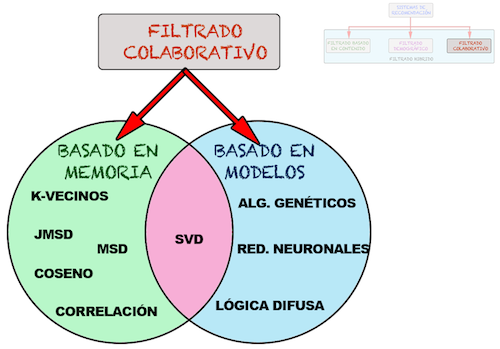
\includegraphics[scale=0.9]{./Imagenes/img02}		
		 			\end{center}
		 		\end{figure}
	 			
	 			\begin{enumerate}[a.]
	 				\item Estrategias basadas en memoria.\\
	 				\\
	 				A las que también se las llama estrategias basadas en vecinos. Son las que hacen recomendaciones basándose en las valoraciones realizadas por los usuarios del sistema. Han sido las estrategias más ampliamente usadas en la implementación de sistemas recomendadores de filtrado colaborativo. Dentro de estas técnicas, existen dos subconjuntos: 
	 				
	 				\begin{itemize}
	 					\item Basado en usuario: se predice la valoración de un usuario para un producto, teniendo en cuenta las valoraciones que han hecho los vecinos del usuario (aquellos usuarios que han valorado de forma parecida los mismos productos que él) para ese mismo producto. \\

	 					\item Basado en producto: se predice la valoración de un usuario para un producto, teniendo en cuenta las valoraciones que ha hecho ese usuario para vecinos del producto (aquellos productos que han sido valorados de forma parecida por los usuarios). 
	 				\end{itemize}
	 				\newpage
	 				\item Estrategias basadas en modelos. \\
	 				\\
	 				El problema de las estrategias basadas en vecinos es que la complejidad de cálculo es enorme. Es por esto por lo que surgieron las estrategias basadas en modelos, con las que se construyen modelos estadísticos de patrones de valoración de usuarios y productos para hacer predicciones automáticas de valoraciones. Con ellas se realiza un preprocesamiento offine de los datos de la 15 plataforma para hacer las recomendaciones y predicciones con esos datos. Entre ellos se encuentran los modelos de semántica latente, redes neuronales o probabilísticos, pero el que más destaca es el modelo de los factores latentes. Es el método más utilizado por la mejora de precisión que ha proporcionado gracias a la utilización de la técnica de factorización de matrices. Lo que hace esta técnica es categorizar usuarios o productos en unas determinadas clases deducidas de las valoraciones aportadas por los usuarios.
	 				
	 			\end{enumerate}
 						
		 		
		 	\end{enumerate}
	 		Aunque los algoritmos de filtrado colaborativo sean el tipo de sistema recomendador más utilizado y popular por la eficacia de sus recomendaciones aún tienen debilidades que provocan que las recomendaciones no sean totalmente efectivas y que, por lo tanto, es necesario que se solventen. Por un lado, tenemos dispersión: el conjunto de valoraciones usuario/producto normalmente es menor que el total de valoraciones posibles. Esto diculta encontrar valoraciones realizadas por el vecino del usuario y sobre el vecino del producto.\cite{nro1:Online}
		 
		 \subsubsection{SISTEMA DE RECOMENDACIÓN BASADO EN CONOCIMIENTO }
		 
		 Tanto los sistemas de recomendación basados en contenido como los basados en filtrado colaborativo necesitan gran cantidad de información sobre las interacciones llevadas a cabo por los usuarios del sistema. Como se ha comentado, esto supone un problema cuando aparecen nuevos productos en la plataforma o nuevos usuarios. Los sistemas de recomendación basados en contenido mejoran la eficacia cuando aparecen nuevos productos, pero aun así, siguen produciéndose recomendaciones poco eficaces en este tipo de escenarios. Además, estos métodos son poco adecuados para productos muy personalizados o productos con los que los usuarios no suelen interactuar, como pueden ser, por ejemplo, objetos de lujo o actividades de ocio o turísticas. También, cuando los productos son complejos de describir, es más difícil poder encontrar relaciones entre los productos o con el perfil del usuario.\\
		 \\
		 En general, los sistemas de recomendación basados en conocimiento son muy apropiados en las siguientes situaciones: 
		 
		 \begin{itemize}
		 	\item Cuando los clientes quieren especificar los requisitos en las recomendaciones. 
		 	\item Cuando es difícil obtener las valoraciones o información de interacciones de un determinado tipo de producto debido a la amplia complejidad de dominio del sistema con respecto a la variedad de tipos y opciones de productos. 
		 	\item Cuando se hacen recomendaciones sobre productos que evolucionan muy rápidamente.
		 \end{itemize}
	
		 Por ejemplo, en productos como ordenadores o coches, es difícil que las valoraciones que han sido realizadas por un usuario en un determinado momento tengan validez pasado un cierto tiempo. Los productos evolucionan tan rápidamente que los usuarios no quieren adquirir productos con características anticuadas, aunque en el pasado les hayan gustado.
		 
		 
		 
		\section{ANALISIS: DIFERENCIAS ENTRE LOS PRINCIPALES TIPOS DE SISTEMA DE RECOMENDACIÓN}
		
			\begin{figure}[H]
				\begin{center}
					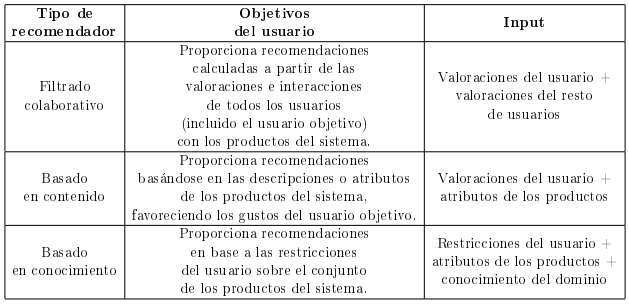
\includegraphics[scale=0.80]{./Imagenes/img03}		
				\end{center}
			\end{figure}
		
		\subsection{PRINCIPALES TAREAS QUE LOS SISTEMAS DE RECOMENDACIÓN}
		
		Las principales tareas que los sistemas de recomendación pueden realizar y por las que los usuarios los utilizan son: 
		
		\begin{itemize}
			\item Ayudar a los usuarios a encontrar productos o usuarios que puedan interesarles. Como se ha comentado al inicio del capítulo, los sistemas de recomendación nos hacen la vida más fácil ayudándonos a elegir entre la amplia oferta que nos proporciona la Web. Es importante mencionar que este tipo de ayuda también se puede aplicar a grupos de personas, cuando es necesario cubrir todas las necesidades de un grupo de personas que buscan un producto. Por ejemplo, cuando un grupo de amigos quiere ir al cine a ver una película, el sistema tiene que cumplir los requisitos y restricciones de los usuarios adaptándolos de la mejor manera posible.
			
			\item Aconsejar al usuario sobre un determinado producto. Si un usuario está interesado en un producto concreto, a través de los sistemas recomendadores, se puede conocer la opinión de la comunidad con respecto a ese producto. Ayudar a encontrar una mezcla de productos nuevos y viejos.
			
			\item Ayudar a encontrar productos nuevos que nos puedan interesar, pero también productos con los que ya hayamos interactuado porque podemos volver a necesitarlo. Por ejemplo, al hacer la lista de la compra podemos volver a comprar alimentos que ya hayamos comprado anteriormente o podemos necesitar comprar productos nuevos para llegar a tener una dieta equilibrada.   
			
			\item Ayudar a encontrar productos según nuestra situación o nuestras necesidades. Es importante que el sistema recomendador nos ofrezca unos productos 11 determinados en la situación en la que lo necesitemos. No es lo mismo necesitar la recomendación de una película para ir a verla con amigos, que para ir a verla con familia. Tampoco es lo mismo necesitar la recomendación de un restaurante para una primera cita que para ir con amigos. De ahí la necesidad de adaptar los sistemas recomendadores para obtener los mejores resultados posibles.
		\end{itemize}
		
	 	
	 	\section{CONCLUSIONES}
	 	
	 	En este trabajo hemos realizado un sistema de recomendaciones utilizando de base la empresa de Airbnb esta empresa ofrece alojamientos a particulares y turísticos mediante la cual los anfitriones pueden publicitar y contratar el arriendo de sus propiedades con sus huéspedes; anfitriones y huéspedes pueden valorarse mutuamente, como referencia para futuros usuarios. \\
	 	\\
	 	Esto se pudo realizar gracias a la herramienta de Colab y archivos csv, que nos permitieron como base de datos para poder generar gráficos de tablas específicas, o información que deseemos poder visualizar.
	 	
	 	
	 	\bibliographystyle{plain}
	 	\bibliography{BIBLIO}
	 		
\end{document}